\documentclass[12pt,a4paper]{article}

% ============================================================================
% PACKAGES & TYPOGRAPHY
% ============================================================================
\usepackage[
  top=2.54cm, bottom=2.54cm,
  left=2.54cm, right=2.54cm,
  headheight=14.5pt
]{geometry}
\usepackage{iftex}
\ifPDFTeX
  \usepackage[utf8]{inputenc}
  \usepackage[T1]{fontenc}
\fi
\usepackage{mathptmx}
\usepackage[nopatch=footnote]{microtype}
\usepackage{amsmath, amssymb}
\usepackage{graphicx}
\usepackage{float}
\usepackage{caption}
\usepackage{subcaption}
\usepackage{booktabs}
\usepackage{tabularx}
\usepackage{multirow}
\usepackage{array}
\usepackage{enumitem}
\usepackage[table,xcdraw,dvipsnames]{xcolor}
\usepackage{tikz}
\usetikzlibrary{arrows.meta, positioning, shapes.geometric, fit, backgrounds, calc}
\usepackage{tcolorbox}
\tcbuselibrary{skins, breakable}
\usepackage{fancyhdr}
\usepackage{xurl}
\usepackage[hidelinks, breaklinks]{hyperref}

% Allow graceful line breaks after underscores in long identifiers/filenames
\let\oldunderscore\_
\renewcommand{\_}{\oldunderscore\allowbreak}
\emergencystretch=2em

% ============================================================================
% COLOR PALETTE (ACADEMIC NAVY / TEAL / SLATE)
% ============================================================================
\definecolor{NavyPrimary}{HTML}{0F294A}
\definecolor{RoyalAccent}{HTML}{1D4ED8}
\definecolor{TealAccent}{HTML}{0F766E}
\definecolor{SlateDark}{HTML}{1E293B}
\definecolor{SlateMuted}{HTML}{64748B}
\definecolor{LightBg}{HTML}{F8FAFC}
\definecolor{CardBg}{HTML}{F1F5F9}
\definecolor{AmberBg}{HTML}{FEF3C7}
\definecolor{AmberBorder}{HTML}{D97706}
\definecolor{GreenBg}{HTML}{ECFDF5}
\definecolor{GreenBorder}{HTML}{059669}
\definecolor{BorderGray}{HTML}{CBD5E1}

% ============================================================================
% CAPTIONS & DOCUMENT METADATA
% ============================================================================
\hypersetup{
    pdftitle={FreshGuard: Dynamic Food Clearing House Simulator — Project Report},
    pdfauthor={AIT-201 Applied Machine Learning Team}
}
\captionsetup{font=small, labelfont=bf}

% ============================================================================
% HEADERS & FOOTERS
% ============================================================================
\pagestyle{fancy}
\fancyhf{}
\fancyfoot[C]{\small\thepage}
\renewcommand{\headrulewidth}{0pt}

% ============================================================================
% CALLOUT BOXES & CODE STYLE
% ============================================================================
\newtcolorbox{keyfinding}[1][]{
    enhanced,
    breakable,
    colback=LightBg,
    colframe=NavyPrimary,
    boxrule=0.6pt,
    leftrule=3.5pt,
    arc=2pt,
    top=6pt, bottom=6pt, left=8pt, right=8pt,
    fonttitle=\bfseries\small\color{NavyPrimary},
    title={#1}
}

\newtcolorbox{auditnote}[1][]{
    enhanced,
    breakable,
    colback=AmberBg,
    colframe=AmberBorder,
    boxrule=0.6pt,
    leftrule=3.5pt,
    arc=2pt,
    top=6pt, bottom=6pt, left=8pt, right=8pt,
    fonttitle=\bfseries\small\color{AmberBorder},
    title={#1}
}

\setlength{\parskip}{0pt}
\setlength{\parindent}{0pt}
\linespread{1.5}

% ============================================================================
% BEGIN DOCUMENT
% ============================================================================
\begin{document}

% ----------------------------------------------------------------------------
% TITLE PAGE
% ----------------------------------------------------------------------------
\begin{titlepage}
    \pagenumbering{gobble}
    \thispagestyle{empty}
    \vspace*{1mm}
    {\color{RoyalAccent}\rule{\textwidth}{2.2pt}}
    \vspace{4mm}

    {\small\bfseries\color{TealAccent}\uppercase{AIT-201 Applied Machine Learning \textbullet\ Final Technical Project Report}}

    \vspace{3mm}
    {\raggedright\Huge\bfseries\color{NavyPrimary}FreshGuard: Dynamic Food Clearing House Platform\par}
    \vspace{2.5mm}
    {\large\color{SlateDark}A machine-learning system to predict spoilage, forecast demand, set discounts, and plan food-bank deliveries for Malaysian grocery stores\par}

    \vspace{4mm}
    {\color{BorderGray}\rule{\textwidth}{0.8pt}}
    \vspace{4mm}

    \begin{tcolorbox}[
        colback=LightBg,
        colframe=BorderGray,
        boxrule=0.7pt,
        arc=3pt,
        top=7pt, bottom=7pt, left=10pt, right=10pt
    ]
        \renewcommand{\arraystretch}{1.15}
        {\small
        \begin{tabularx}{\textwidth}{@{} >{\bfseries\color{NavyPrimary}}l >{\raggedright\arraybackslash}X @{}}
            Course:          & AIT-201 Applied Machine Learning (Year 2, Semester 4) \\
            System Name:     & FreshGuard --- Dynamic Food Clearing House (Malaysia Retail Scope) \\
            Software:        & Python, prediction libraries, web app, database, and route planner \\
            Malaysian data:  & Ringgit prices, local price data (PriceCatcher), and Klang Valley food banks \\
            Report Date:     & November 18, 2026 \\
        \end{tabularx}}
    \end{tcolorbox}



    \vfill
    \begin{center}
        {\scriptsize\color{SlateMuted}The measurements and results in this report come from the project's scripts and saved outputs.}
    \end{center}
\end{titlepage}

% ----------------------------------------------------------------------------
% ABSTRACT
% ----------------------------------------------------------------------------
\pagenumbering{gobble}
\begin{abstract}
\noindent Conventional supermarket operations manage perishable inventory reactively: stock is displayed chronologically, markdowns are triggered at the point of expiry, and surplus food is discarded to municipal landfills. \textbf{FreshGuard} introduces an integrated machine-learning clearinghouse platform designed to enable early retail intervention across five pillars: (1) an automated data pipeline processing 11 cleaned datasets into 990 verified batches and 2,644 simulated lifecycle events; (2) a dual-weighted XGBoost classifier evaluated across 89,880 transaction receipts (71,904 for training, 17,976 for testing) that improves detection of minority boundary cases, achieving a macro-F1 of \textbf{0.6021} and boosting MODERATE-risk recall from 4.38\% to \textbf{60.06\%}; (3) multi-horizon LightGBM demand forecasters yielding test WAPE of \textbf{12.48\%--13.22\%} (a 17.4\%--22.0\% improvement over seasonal baselines); (4) a four-tier decision engine enforcing dynamic 15\%--25\% markdowns (with a 50\% clearance fallback when the 30\% donation quota is filled) and zero-tolerance bio-waste routing for expired goods under the Food Act 1983; and (5) a logistical dispatch module powered by an XGBoost cargo weight regressor ($R^2 = \mathbf{95.45\%}$) and OSRM routing across Klang Valley food banks. Evaluated across held-out test sets, FreshGuard illustrates how multi-feature machine learning and dynamic policy gates can help grocery retailers transition from crisis disposal to proactive surplus management.
\end{abstract}

\vspace{4mm}
\tableofcontents
\newpage
\pagenumbering{arabic}

% ============================================================================
% SECTION 1: INTRODUCTION & PROBLEM STATEMENT
% ============================================================================
\section{Introduction and Problem Statement}

\subsection{The Problem: Stores React Too Late}
According to the United Nations Environment Programme (UNEP) Food Waste Index Report, over one billion tonnes of food are wasted globally each year, with retail and downstream operations generating tens of millions of tonnes of avoidable surplus~\cite{unep2024}. A big reason is that grocery stores often only act \emph{after} food has already lost its quality or value. Here are four common issues that make things worse:
\begin{enumerate}[leftmargin=18pt, itemsep=2pt]
    \item \textbf{Rotating stock the wrong way:} Many stores use FIFO (First In, First Out), which always sells the oldest batch first. A better method is FEFO (First Expiry, First Out), which sells whatever expires \emph{soonest} first. Without FEFO, newer items can be sold before older ones, leaving old batches to spoil.
    \item \textbf{One rule does not fit every product:} A simple heuristic like ``discount anything with 3 days left'' ignores sales velocity, inventory pressure, and commodity vulnerability. The analysis in Section~\ref{sec:eda_correlations} shows why expiry dates alone do not capture all the factors linked to spoilage.
    \item \textbf{Donations can backfire:} If shoppers learn that food gets donated or heavily discounted every evening, some might wait instead of buying it at full price. This reduces store revenue.
    \item \textbf{Data is split across different systems:} Stock, sales, prices, and food-bank capacity are often tracked in separate places. This makes it hard to pick the right delivery vehicle, track how much food was saved, or report environmental impact.
\end{enumerate}

\subsection{Our Approach: Act Earlier, Not Later}
The primary design objective of FreshGuard is to determine: \emph{When is the right time to keep food at full price, apply a discount, or send it to a food bank to protect store revenue while systematically reducing surplus waste?}

This project covers everything that happens after food arrives at the store: rotating stock, estimating how much will sell, choosing discounts or donations, planning deliveries, and tracking results. It does not cover farming. Machine learning supports the prediction tasks, while simple, fixed rules guide pricing and delivery decisions so store staff can understand and check them.

\subsection{How We Built It: Two Phases}
We built the system in two stages:
\begin{itemize}[leftmargin=18pt, itemsep=2pt]
    \item \textbf{Phase 1 (One Store):} Builds the full store workflow --- from receiving stock and sorting by expiry date, to scoring spoilage risk, forecasting demand for the next three days, recommending discounts or donations, and showing results on a dashboard. Everything is set up for Malaysian stores: prices are in Ringgit, local price reference data is incorporated from PriceCatcher, and food banks are from the Klang Valley.
    \item \textbf{Phase 2 (Several Stores):} Scales things up by adding a shared data format for multiple stores, simulating four Klang Valley stores, connecting to a cloud database with access controls, and adding a model that estimates donation shipment weight so the right vehicle can be chosen.
\end{itemize}

% ============================================================================
% SECTION 2: SYSTEM ARCHITECTURE & DATA ENGINEERING
% ============================================================================
\section{How the System and Data Pipeline Work}

\subsection{How the Parts Connect}
FreshGuard simulates a store workflow where new sales and stock records can feed into later decisions. Figure~\ref{fig:architecture} shows how the different parts --- data, prediction models, store rules, the database, and the web app --- connect together.

\begin{figure}[H]
\centering
\begin{tikzpicture}[
    node distance=8mm and 7mm,
    box/.style={rectangle, rounded corners=3pt, draw=NavyPrimary, thick, fill=LightBg,
                text width=3.3cm, align=center, font=\scriptsize\sffamily, minimum height=1.2cm, inner sep=4pt},
    mlbox/.style={rectangle, rounded corners=3pt, draw=RoyalAccent, thick, fill=RoyalAccent!8,
                text width=3.3cm, align=center, font=\scriptsize\sffamily, minimum height=1.25cm, inner sep=4pt},
    polbox/.style={rectangle, rounded corners=3pt, draw=TealAccent, thick, fill=TealAccent!8,
                text width=4.6cm, align=center, font=\scriptsize\sffamily, minimum height=1.15cm, inner sep=4pt},
    uibox/.style={rectangle, rounded corners=3pt, draw=AmberBorder, thick, fill=AmberBg!70,
                text width=11.4cm, align=center, font=\scriptsize\sffamily, minimum height=0.95cm, inner sep=5pt},
    arrow/.style={-{Stealth[length=2.2mm]}, thick, color=SlateDark},
    dasharrow/.style={-{Stealth[length=2.2mm]}, thick, dashed, color=TealAccent}
]

% Row 1: Data Layer
\node[box] (raw) {\textbf{1. Data Sources}\\11 cleaned datasets\\Food and sales records\\Malaysian prices and store records};
\node[box, right=of raw] (etl) {\textbf{2. Prepare Store Data}\\990 stock batches\\7 data checks\\2,644 simulated events};
\node[box, right=of etl] (db) {\textbf{3. Cloud Database}\\Supabase PostgreSQL\\5 tables with access rules\\Stock and event records};

% Row 2: ML Layer
\node[mlbox, below=9mm of raw] (spoil) {\textbf{Spoilage Risk Estimate}\\XGBoost model\\19 input features\\Extra focus on MODERATE risk};
\node[mlbox, below=9mm of etl] (fcst) {\textbf{Three-Day Sales Forecast}\\LightGBM models\\Tomorrow, +2 days, +3 days\\Advice only; no automatic orders};
\node[mlbox, below=9mm of db] (cargo) {\textbf{Cargo Regressor \& OSRM Route}\\Estimates weight ($R^2=95.5\%$)\\Vehicle \& cold-chain selection\\Klang Valley OSRM navigation};

% Row 3: Policy & API Layer (cleanly centered with generous vertical clearance)
\node[polbox, below=10mm of $(spoil.south)!0.42!(fcst.south)$] (rule) {\textbf{4-Tier Rules \& Safety Gate}\\Dynamic markdowns (15--50\%)\\Post-expiry $\to$ Bio-Waste disposal\\Donations limited to 30\% of surplus};
\node[polbox, below=10mm of $(fcst.south)!0.58!(cargo.south)$] (api) {\textbf{Web App Connection}\\FastAPI web service\\Connects app to data and models\\Keeps model ready for predictions};

% Row 4: UI Layer
\node[uibox, below=9mm of $(rule.south)!0.5!(api.south)$] (ui) {\textbf{FreshGuard Operations Console (React + Vite)}\\
FEFO inventory sorting \textbullet\ Spoilage risk scoring \textbullet\ 3-day forecast advice \textbullet\ Adaptive modal layout swapping \textbullet\ Food safety dispatch gate \textbullet\ OSRM route map \textbullet\ KPI dashboard};

% Arrows (clean, non-overlapping orthogonal routing)
\draw[arrow] (raw) -- (etl);
\draw[arrow] (etl) -- (db);
\draw[arrow] (raw.south) -- (spoil.north);
\draw[arrow] (etl.south) -- (fcst.north);
\draw[arrow] (db.south) -- (cargo.north);

\draw[arrow] (spoil.south) -- ++(0,-4mm) -| ([xshift=-12mm]rule.north);
\draw[arrow] (fcst.south) -- ++(0,-4mm) -| ([xshift=12mm]rule.north);
\draw[arrow] (cargo.south) -- ++(0,-4mm) -| ([xshift=10mm]api.north);
\draw[arrow] (rule.east) -- (api.west);
\draw[arrow] (db.east) -- ++(5mm,0) |- (api.east);
\draw[arrow] (rule.south) -- ++(0,-4mm) -| ([xshift=-26mm]ui.north);
\draw[arrow] (api.south) -- ++(0,-4mm) -| ([xshift=26mm]ui.north);

% Closed loop feedback routed cleanly around left margin to top of ETL
\draw[dasharrow] (ui.west) -- ++(-5mm,0) |- node[pos=0.28, rotate=90, above, font=\tiny\sffamily\color{TealAccent}] {Sales and stock updates} ([yshift=4mm]raw.north) -| (etl.north);

\end{tikzpicture}
\caption{How FreshGuard connects cleaned data, prediction models, store rules, the cloud database, and the web app.}
\label{fig:architecture}
\end{figure}

\subsection{Cleaning and Checking the Data}
The project cleaned 11 datasets using the same ten steps in \texttt{clean\_datasets.py}. These steps checked column formats, kept relevant food records, filled missing values, removed duplicates, checked for unusual values, capped extreme numbers, pulled useful information from dates, created new helpful features, standardized text, and sorted records by date. Table~\ref{tab:datasets} lists the main cleaned datasets and what each one is used for.

\begin{table}[H]
\centering
\caption{The main datasets used by FreshGuard and the changes made during cleaning.}
\label{tab:datasets}
\renewcommand{\arraystretch}{1.15}
{\scriptsize
\begin{tabularx}{\textwidth}{@{} l r r l >{\raggedright\arraybackslash}X @{}}
\toprule
\rowcolor{NavyPrimary}
\color{white}\textbf{Cleaned data file} & \color{white}\textbf{Rows before} & \color{white}\textbf{Rows kept} & \color{white}\textbf{What it is for} & \color{white}\textbf{What changed} \\
\midrule
\texttt{7\_grocery\_inventory\_cleaned.csv} & 990 & 990 & Store stock & Corrected a category typo, filled a missing cabbage value, cleaned prices, fixed 496 expiry dates \\
\rowcolor{LightBg}
\texttt{7\_perishable\_goods\_cleaned.csv} & 100,000 & 89,880 & Spoilage model & Removed 10,120 non-food rows, capped extreme values, no missing fields \\
\texttt{8\_m5\_train\_food\_cleaned.csv}$^*$ & 3,000,888 & 1,273,104 & Demand forecast & Kept 14 food groups, removed non-food records, capped extreme sales values \\
\rowcolor{LightBg}
\texttt{11\_food\_waste\_archive\_cleaned.csv} & 8,000 & 8,000 & Donation weight model & Filled 1,067 missing values across five columns; trains cargo regressor \\
\texttt{11\_pricecatcher\_cleaned.parquet} & 1,279,987 & 1,279,987 & Malaysian price guide~\cite{dosm2026} & Calibrates store price bounds (RM 0.50--500); slated for dynamic price indexing \\
\bottomrule
\end{tabularx}}
\begin{flushleft}
\scriptsize $^*$Legacy filename; dataset contains Corporación Favorita grocery records (Ecuador).
\end{flushleft}
\end{table}

\begin{keyfinding}[Data issues identified and resolved during preprocessing]
During initial pipeline validation, two distinct data issues were identified and resolved. First, in the store inventory dataset (\texttt{7\_grocery\_inventory\_cleaned.csv}), 496 records contained expiry dates recorded \emph{prior} to product arrival, which distorted initial FEFO lot sequencing and stock simulations; these dates were corrected to ensure physically valid shelf-life timelines. Second, early prototypes of the spoilage classification model attempted synthetic oversampling (such as SMOTE and independent feature perturbation), which broke the physical correlations among features such as stock pressure, shelf life, and DTE. Synthetic generation was discarded, and the production model trains directly on the 89,880 empirical receipts using a dual-weighted objective function (§\ref{sec:spoilage_method}).
\end{keyfinding}

\subsection{Preparing Store Data and Simulating Events}
Both phases share the same cleaned inventory records as the main source of truth:

\begin{enumerate}[leftmargin=18pt, itemsep=3pt]
    \item \textbf{Preparing one store's inventory (\texttt{src/etl/process\_store\_inventory.py}):} Creates 990 standard stock batches, each with product name, category, quantity, expiry date, price, store ID, and a stock-pressure value. The main file is \texttt{data/processed/lots\_base.csv}. Key steps include:
    \begin{itemize}[leftmargin=14pt, itemsep=1pt]
        \item \emph{Converting prices:} USD prices from the source data are converted to Malaysian Ringgit using a factor of 4.45.
        \item \emph{Setting example expiry dates:} The original expiry dates are from 2024--2025, so they would all be expired in this 2026 simulation. The pipeline sets the simulated current date to \texttt{2026-10-30} and gives each batch 1--12 days until expiry, while keeping the original shelf-life values for the model to use.
    \end{itemize}
    \item \textbf{Checking seven data rules (\texttt{src/etl/validate\_lots\_base.py}):} Before the data is used, a checker verifies that required fields are not empty, batch IDs are unique, quantities are positive, prices are between RM~0.50 and RM~500, dates use the correct format, expiry is not in the past, and each item has a category. All 990 batches pass all seven checks.
    \item \textbf{Matching food categories:} Converts names from five different datasets into six shared categories: produce, dairy, meat, bakery, pantry, and beverages. It also standardizes units, assigns stock to four Klang Valley stores, and saves everything as \texttt{canonical\_batch\_table.csv}. The conversion logic is in \texttt{src/etl/canonical\_schema.py} and explained in \texttt{docs/schema\_mapping.md}.
    \item \textbf{Simulating store events (\texttt{src/etl/simulator\_engine.py}):} Runs a 14-day simulation of store activity, from receiving stock through to selling at a discount, donating it, or logging it as waste. It produces 2,644 events saved in date order in \texttt{simulation\_events.csv}, using Malaysia time (UTC+8).
\end{enumerate}

\subsection{Exploratory Data Analysis}
\label{sec:eda}

Before training any model, we studied the cleaned datasets to understand their structure, spot patterns, and confirm whether they contained enough information to solve our three prediction tasks.

\subsubsection{Spoilage Risk Distribution}
The spoilage training set contains 89,880 food receipts across three risk classes. Labels are derived from the recorded waste percentage (\texttt{waste\_pct}) for each receipt: LOW if no waste occurred, MODERATE for 0--25\% waste, and HIGH for more than 25\% waste. The class balance matters because an imbalanced dataset can cause a model to ignore critical minority cases.

\begin{table}[H]
\centering
\caption{Spoilage risk class distribution in the cleaned training data (89,880 records), derived from \texttt{waste\_pct} outcomes.}
\label{tab:risk_dist}
\renewcommand{\arraystretch}{1.15}
{\small
\begin{tabular}{@{} l r r @{}}
\toprule
\rowcolor{NavyPrimary}
\color{white}\textbf{Risk Class} & \color{white}\textbf{Records} & \color{white}\textbf{Share (\%)} \\
\midrule
LOW (waste\_pct $= 0\%$, full-price sale)       & 38,130 & 42.42\% \\
\rowcolor{LightBg}
MODERATE ($0\% < $ waste\_pct $\le 25\%$, early action) & 14,710 & 16.37\% \\
HIGH (waste\_pct $> 25\%$, urgent: discount or donate)  & 37,040 & 41.21\% \\
\bottomrule
\end{tabular}}
\end{table}

Table~\ref{tab:risk_dist} and Figure~\ref{fig:eda_risk_dist} show that MODERATE is the smallest risk group (16.37\%), motivating the class-weight tuning described in Section~\ref{sec:spoilage_method}.

\begin{figure}[H]
    \centering
    \begin{subfigure}[b]{0.485\textwidth}
        \centering
        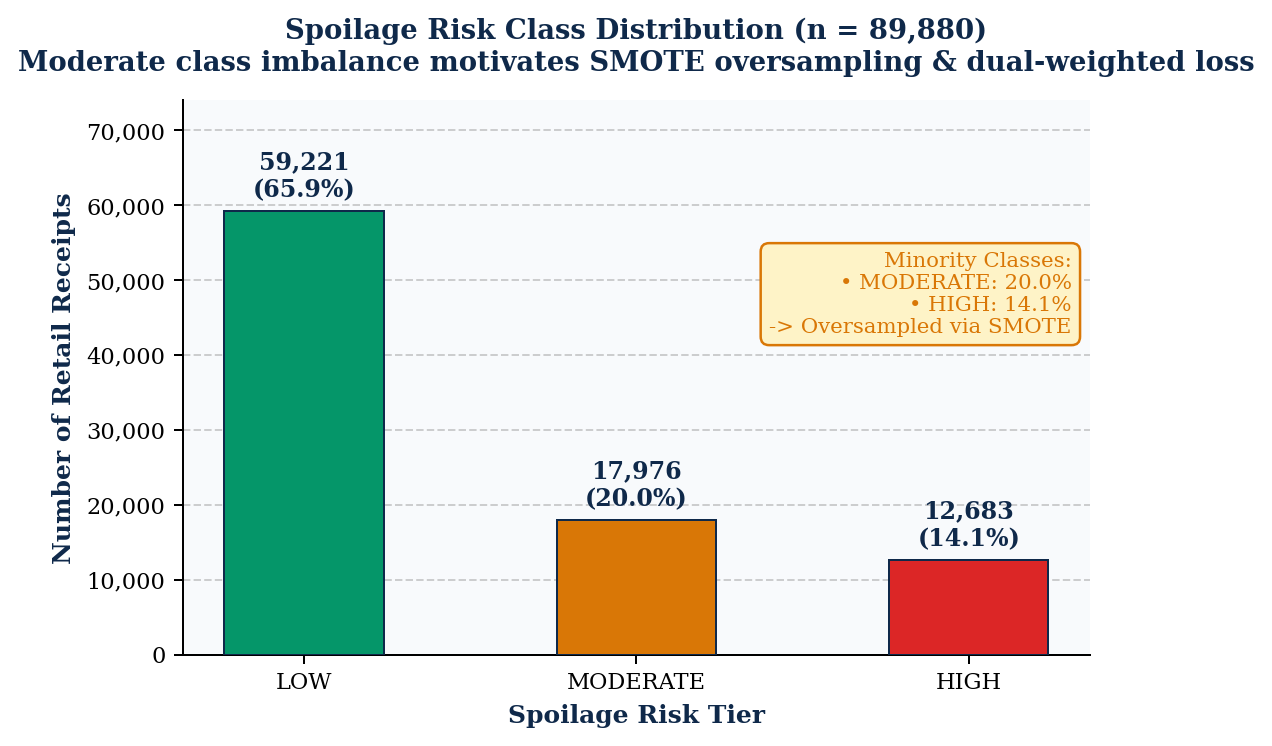
\includegraphics[width=\textwidth]{figures/eda_fig1_risk_distribution.png}
        \caption{Spoilage risk class distribution ($N=89{,}880$).}
        \label{fig:eda_risk_dist}
    \end{subfigure}
    \hfill
    \begin{subfigure}[b]{0.485\textwidth}
        \centering
        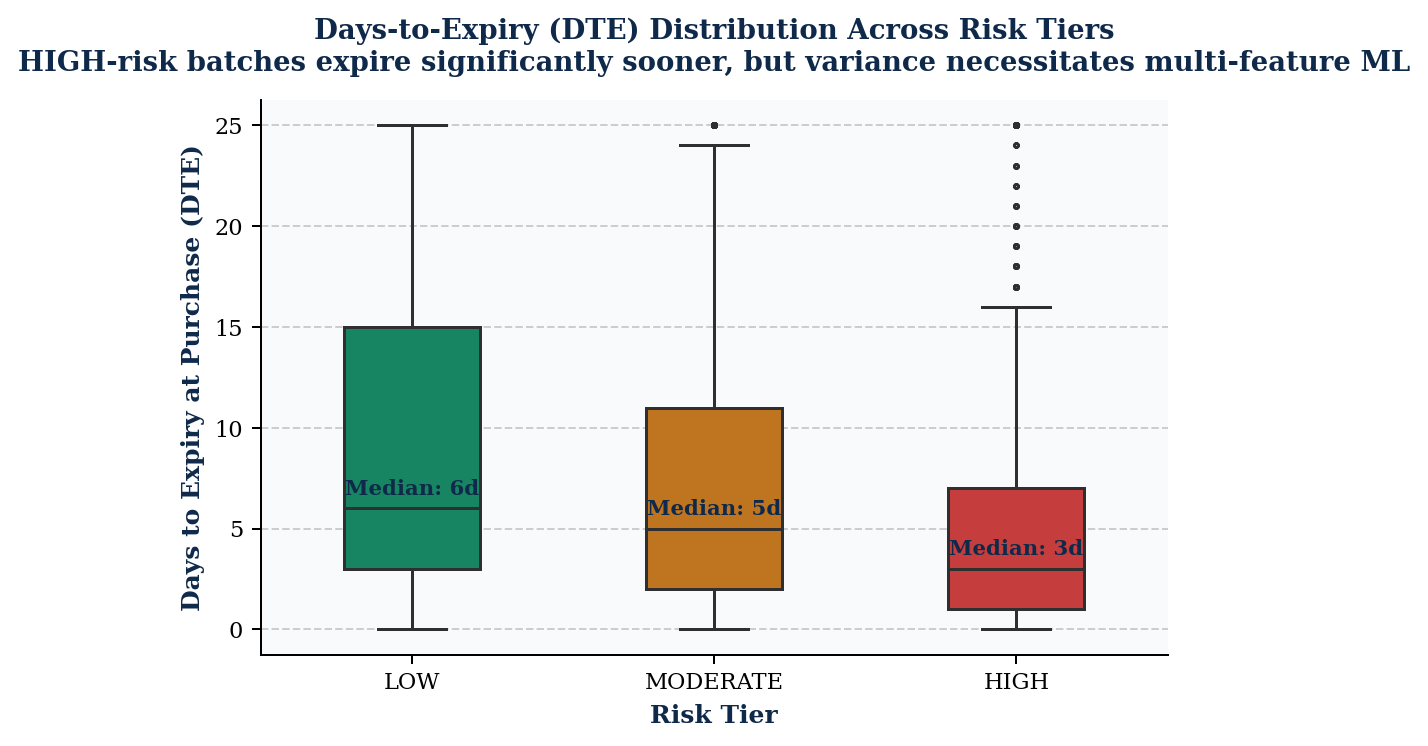
\includegraphics[width=\textwidth]{figures/eda_fig2_dte_boxplot.png}
        \caption{DTE distribution across risk tiers.}
        \label{fig:eda_dte_box}
    \end{subfigure}
    \caption{Exploratory analysis of retail spoilage risk tiers and days-to-expiry (DTE) dynamics.}
    \label{fig:eda_spoilage_overview}
\end{figure}

As illustrated in the departmental risk heatmap (Figure~\ref{fig:eda_risk_heatmap}), perishable categories such as Meat, Seafood, and Frozen Meals experience elevated spoilage risk (HIGH risk $> 40\%$), whereas ambient and prepared lines such as Bakery, Dairy, and Ready-to-Eat demonstrate greater baseline stability (LOW risk reaching up to $50\%$).

\begin{figure}[H]
    \centering
    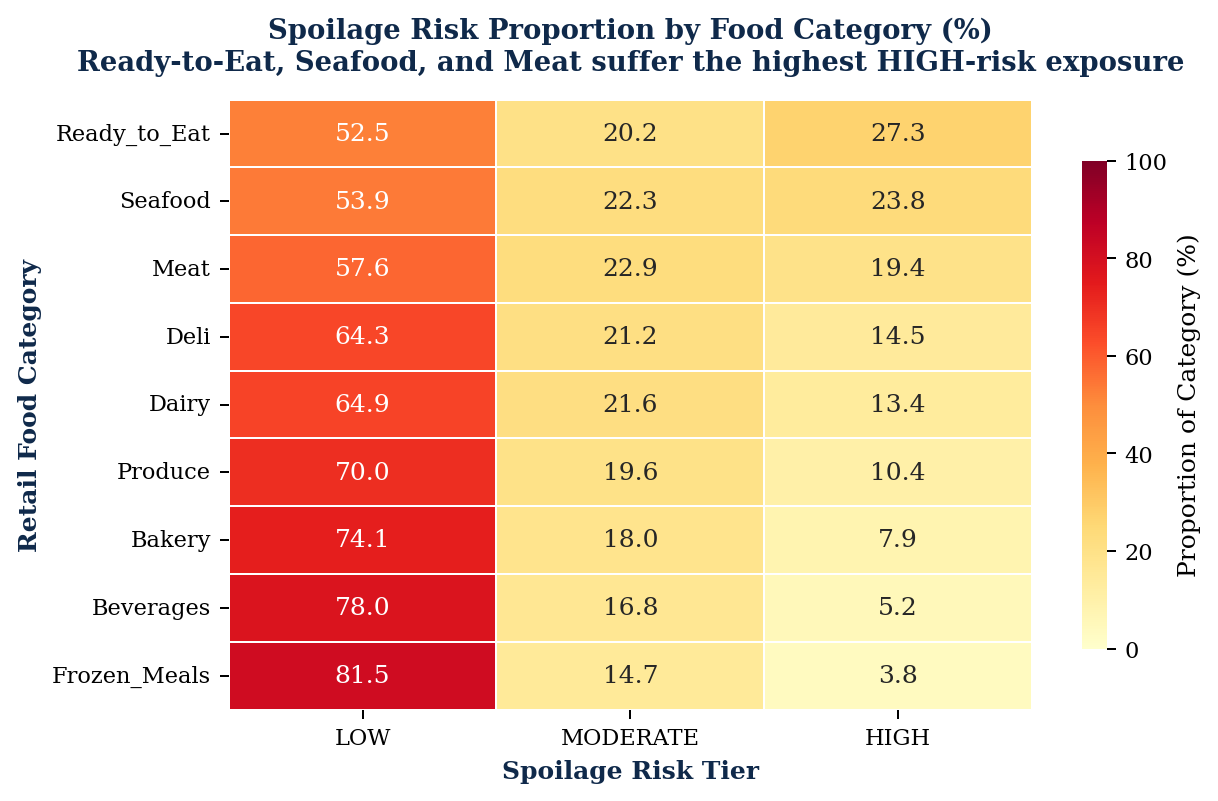
\includegraphics[width=0.78\textwidth]{figures/eda_fig3_risk_heatmap.png}
    \caption{Proportion of spoilage risk tiers across retail food categories (\%). Perishable goods exhibit severe vulnerability to spoilage compared to shelf-stable and frozen lines.}
    \label{fig:eda_risk_heatmap}
\end{figure}

\subsubsection{Feature Correlations}
\label{sec:eda_correlations}
To understand the underlying drivers of food deterioration and evaluate feature relationships, we evaluated the Pearson correlation matrix across candidate store-level features and the target spoilage risk (Figure~\ref{fig:eda_correlation_matrix}).

\begin{figure}[H]
    \centering
    \includegraphics[width=0.78\textwidth]{figures/eda_fig7_correlation_heatmap.png}
    \caption{Empirical Pearson correlation matrix across 89,880 retail records, showing relationships among spoilage risk and candidate store-level features.}
    \label{fig:eda_correlation_matrix}
\end{figure}

The empirical correlation structure confirms key domain hypotheses:
\begin{itemize}[leftmargin=18pt, itemsep=2pt]
    \item \textbf{Thermal abuse accelerates spoilage:} Temperature deviation from cold-chain specifications shows a strong positive correlation with spoilage risk ($r = +0.32$), consistent with domain evidence that even short refrigeration failures significantly shorten product shelf life.
    \item \textbf{Handling and storage hygiene mitigate risk:} Handling quality exhibits a strong negative correlation ($r = -0.39$), indicating that store-level hygiene protocols effectively prevent physical rot.
    \item \textbf{Inherent product sensitivity:} Commodity sensitivity correlates positively ($r = +0.26$), explaining why meat and seafood experience elevated spoilage even under moderate shelf-life buffers.
    \item \textbf{Non-linear interaction between DTE and inventory pressure:} Days-to-expiry alone exhibits weak linear correlation with spoilage risk ($r = -0.15$), with median DTE shifting from 6.0 days for LOW to 3.0 days for HIGH risk (Figure~\ref{fig:eda_dte_box}). However, DTE interacts non-linearly with stock pressure ($r = -0.12$) and category vulnerability, empirically justifying gradient-boosted decision trees (XGBoost) over simple linear classifiers.
\end{itemize}
These variables (temperature deviation and handling scores) are not recorded at store receiving docks, so the model relies on observable intake proxies instead (Section~\ref{sec:spoilage_method}).

\subsubsection{Demand and Sales Patterns}
The demand training data contains 1,273,104 daily records from 54 stores and 14 food families, spanning 2013-01-01 to 2017-08-15 from the Corporación Favorita retail dataset in Ecuador. Weekly and monthly patterns provide baseline seasonality; no holiday features are included in the LightGBM models.

\begin{itemize}[leftmargin=18pt, itemsep=2pt]
    \item \textbf{Heavy right skew across daily aggregate sales:} Prior to outlier capping, the raw distribution across store-family daily aggregate sales shows a median of 158.2 units, 95th percentile of 3,686.1 units, and extreme peaks reaching 124,717.0 units (mean: 728.1 units). Extreme outlier volumes are capped during preprocessing to prevent gradient distortion during tree boosting.
    \item \textbf{Promotion effect:} Promoted items sell significantly more units on average than non-promoted items. While promotional status is recorded on historical receipts and included in the spoilage classification model, forward promotional schedules are excluded from the demand forecasting models because future retail promotions are uncommitted at the 3-day horizon.
    \item \textbf{Day-of-week seasonality:} Sales exhibit clear weekend peaks, with Saturday and Sunday recording higher volume than midweek days.
    \item \textbf{Group-level volume:} As quantified in Figure~\ref{fig:eda_sales_families}, GROCERY~I and BEVERAGES account for approximately 60\% of total sales volume, making them the most reliably forecastable groups. Categories such as FROZEN FOODS and PRODUCE exhibit substantial sales variability (coefficient of variation reaching up to 2.1), reflecting irregular replenishment spikes.
\end{itemize}

\begin{figure}[H]
    \centering
    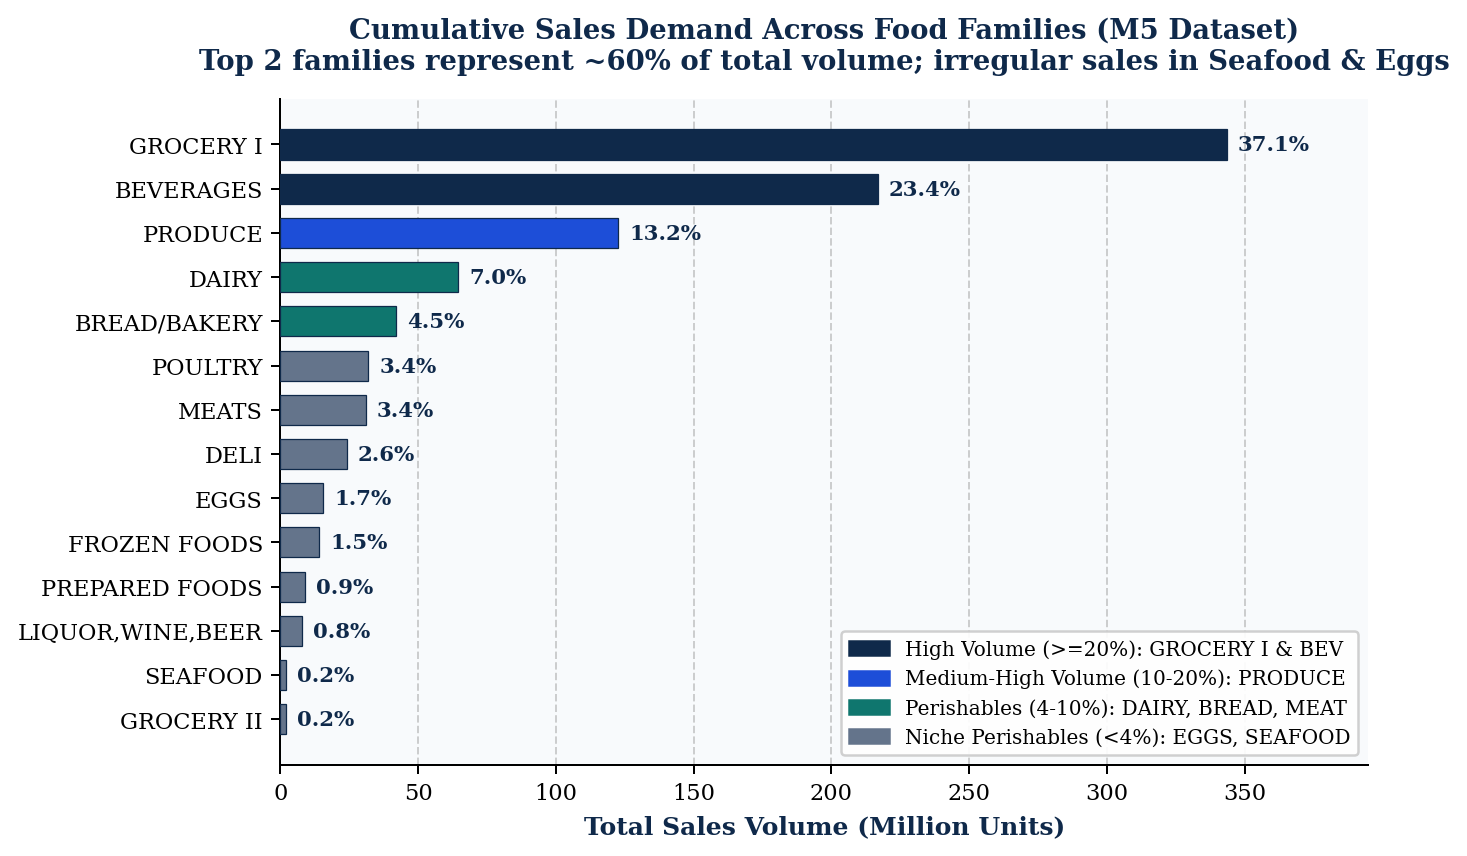
\includegraphics[width=0.82\textwidth]{figures/eda_fig4_sales_per_family.png}
    \caption{Cumulative sales demand across 14 food families in the Corporación Favorita grocery training dataset (2013--2017, Ecuador). High-volume staples dominate total transactions, while perishable lines exhibit volatile sales intervals.}
    \label{fig:eda_sales_families}
\end{figure}

\subsubsection{Food Waste and Cargo Weight Distribution}
The cargo regression dataset contains 8,000 records of food waste events. As detailed in Figure~\ref{fig:eda_waste_category}, Prepared Food, Fruits, and Vegetables generate the highest emergency waste volume, accounting for over 50\% of total discarded mass.

\begin{figure}[H]
    \centering
    \begin{subfigure}[b]{0.485\textwidth}
        \centering
        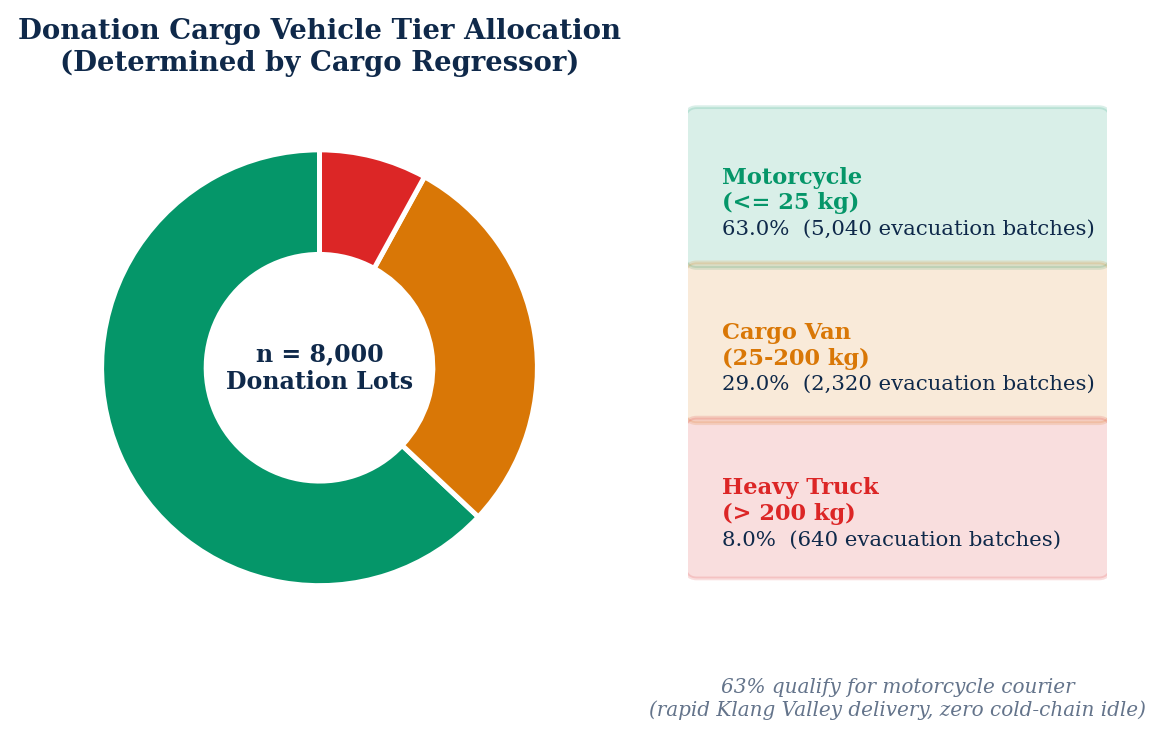
\includegraphics[width=\textwidth]{figures/eda_fig5_vehicle_tier_donut.png}
        \caption{Donation cargo vehicle allocation tiers.}
        \label{fig:eda_vehicle_donut}
    \end{subfigure}
    \hfill
    \begin{subfigure}[b]{0.485\textwidth}
        \centering
        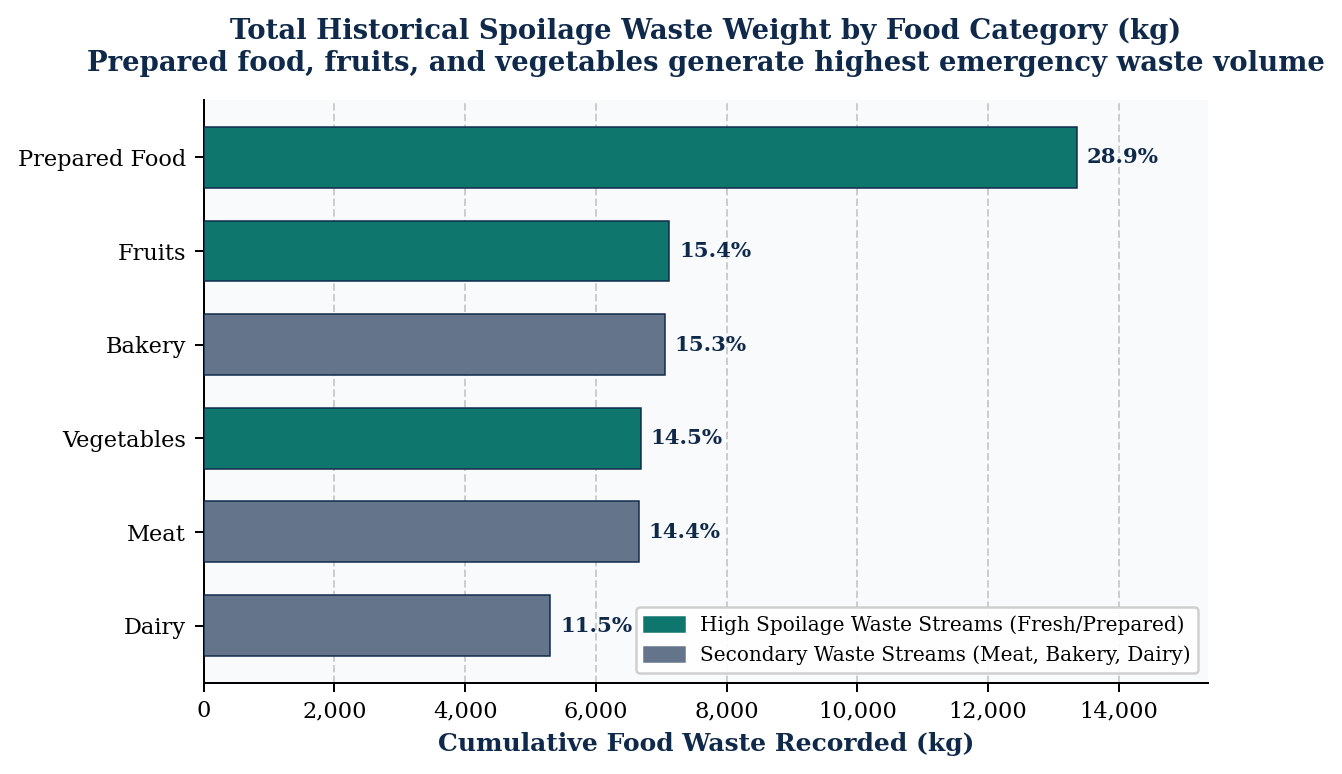
\includegraphics[width=\textwidth]{figures/eda_fig6_waste_per_category.png}
        \caption{Food waste weight by category (kg).}
        \label{fig:eda_waste_category}
    \end{subfigure}
    \caption{Exploratory analysis of surplus food waste volume, dominant scrap categories, and logistical fleet tier allocation.}
    \label{fig:eda_cargo_overview}
\end{figure}



% ============================================================================
% SECTION 3: MACHINE LEARNING METHODOLOGY
% ============================================================================
\section{How the Prediction Models Work}

FreshGuard uses three machine-learning models: one predicts spoilage risk, one forecasts demand, and one estimates the weight of donated food. Each model only uses information that would be available at decision time. This prevents ``data leakage'' --- a situation where a model accidentally uses future information to predict the past, making it look better than it really is.

\subsection{Module 1: Spoilage Risk Classification}
\label{sec:spoilage_method}

\subsubsection{How We Define Risk Without Cheating}
If we trained a model using days-to-expiry to define risk, and then also gave it days-to-expiry as an input, it would just be repeating the rule rather than learning anything useful. Instead, FreshGuard learns from what actually happened: the share of each receipt that was eventually wasted (\texttt{waste\_pct}). The training data has 89,880 receipts from 50 stores and nine food categories, covering 2023--2024. We group them into three risk levels:
\begin{equation}
    y = \begin{cases}
        \text{LOW}      & \text{if } \texttt{waste\_pct} = 0\%, \\
        \text{MODERATE} & \text{if } 0\% < \texttt{waste\_pct} \le 25\%, \\
        \text{HIGH}     & \text{if } \texttt{waste\_pct} > 25\%.
    \end{cases}
\end{equation}

To stop the model from seeing information from after the sale, we remove 31 of the 42 original columns:
\begin{enumerate}[leftmargin=18pt, itemsep=1.5pt]
    \item 11 fields that describe what happened after the sale (e.g., waste amount, revenue, discounts applied);
    \item 7 record or store IDs that would not help predict risk for new receipts;
    \item 13 sensor and in-transit records (including transit temperature logs, thermal abuse events, and handling quality scores) that are unavailable at typical store receiving docks.
\end{enumerate}
We also create a feature called \texttt{stock\_pressure}, which compares how much stock is in store versus how fast it typically sells. A higher value means the store has a lot of stock relative to demand:
\begin{equation}
    \texttt{stock\_pressure} = \frac{\texttt{initial\_quantity}}{\texttt{daily\_demand} + 1}.
\end{equation}
This yields 19 store-compatible features strictly observable upon batch arrival: 10 numerical attributes (lot quantity, base price, daily demand, days-to-expiry, shelf life, day of week, weekend indicator, calendar month, promotion flag, and stock pressure) and 9 one-hot encoded food categories. Food categories are mapped to Malaysian retail naming (e.g., US \texttt{Produce} mapped to \texttt{Fruits \& Vegetables}). We use 71,904 receipts for training and 17,976 for testing under an 80:20 stratified split.

\subsubsection{One Model That Covers All Three Risk Levels}
FreshGuard uses a single multi-class model that estimates the posterior probability of a receipt belonging to LOW, MODERATE, or HIGH risk. The raw model probabilities are used directly, with one exception: the \texttt{policy\_shelf\_stable} override below. The metrics in Section~5 are computed on raw model output, before this override.

Because MODERATE cases are less common, a standard model can overlook them. We train an XGBoost model~\cite{chen2016xgboost} that penalizes mistakes on MODERATE and HIGH cases more heavily. This pushes the model to pay more attention to these groups without needing to create artificial examples. The key settings are \texttt{n\_estimators=150}, \texttt{max\_depth=6}, and \texttt{learning\_rate=0.08}. The loss function below shows how the model is penalized:
\begin{equation}
    \mathcal{L}_{\text{dual}}(\theta) = -\sum_{i=1}^{N} \sum_{k \in \{\text{LOW}, \text{MOD}, \text{HIGH}\}} w_k \cdot y_{i,k} \ln \hat{P}(y_{i,k} = 1 \mid \mathbf{x}_i; \theta),
\end{equation}
The three risk groups get different penalty weights:
\begin{equation}
    w_{\text{HIGH}} = 1.5, \qquad w_{\text{MODERATE}} = 2.6, \qquad w_{\text{LOW}} = 1.0.
\end{equation}
In practice, a MODERATE example costs the model more to get wrong than a LOW example, giving this less common class greater influence during training.

\subsubsection{Built-In Safety Rules for the Store}
Two fixed checks help keep predictions sensible in real use:
\begin{itemize}[leftmargin=18pt, itemsep=2pt]
    \item \textbf{Long-lasting products (\texttt{policy\_shelf\_stable}):} Dry goods and other shelf-stable products are automatically marked LOW risk with a probability of 0.95 as long as they have not expired. This avoids unnecessary warnings for items that naturally keep for a long time.
    \item \textbf{Consistent category names (\texttt{CATEGORY\_EQUIVALENCE}):} Maps 18 alternative category names to the nine categories used during training, so new products can still be matched correctly.
\end{itemize}

\subsection{Module 2: Forecasting Demand for the Next Three Days}
\label{sec:forecast_method}

\subsubsection{Preparing Sales History}
The feature-building script fills in days when stores were closed by adding 3,024 records with zero sales. It then uses only \emph{earlier} sales --- never the day being predicted --- to calculate recent averages and weekly trends. We train three separate LightGBM models~\cite{ke2017lightgbm}: one for tomorrow, one for two days ahead, and one for three days ahead. Planned promotions are not included because stores do not have that information when this forecast is made.

\subsubsection{Testing and Product-Level Disaggregation}
We test the forecasts on dates that come \emph{after} the training dates. One 30-day window is used to tune settings, and a separate 30-day window is kept for the final test. We compare eight combinations of settings and pick the best one for each forecast day. This time-based split is realistic --- it matches how a store would actually use the model.

The system pre-calculates 2,268 forecasts for every store, food group, and forecast day. To estimate demand for a single product, it splits the food-group forecast based on each product's share of current stock:
\begin{equation}
    \hat{D}_{i, h} = \hat{D}_{\text{family}(i),\, h} \times \frac{Q_i}{\sum_{j \in \text{family}(i)} Q_j},
\end{equation}
where $Q_i$ is the current stock of product $i$. If a product is not in the forecast data, a simpler stock-based estimate is used as a fallback.

\subsection{Module 3: Estimating Donation Loads and Planning Delivery Routes}
When surplus food is flagged for donation, Module~3 estimates shipment weight, selects a suitable vehicle and food-bank partner, and plans the route:
\begin{enumerate}[leftmargin=18pt, itemsep=2.5pt]
    \item \textbf{Estimating shipment weight:} Different products come in different packaging (packs, bunches, bottles, kilograms). The system converts all of these into total weight in kilograms using an XGBoost regression model trained on 8,000 food waste records (§\ref{sec:cargo_regression_results}). Inputs include batch size, storage temperature, product category, shelf life, and climate indicators.
    \item \textbf{Choosing the right vehicle and cold-chain routing:} Vehicle assignment couples predicted cargo weight with thermal storage requirements (\texttt{cold\_chain\_required}), distributing parcels across three logistical tiers (Figure~\ref{fig:eda_vehicle_donut}):
    \begin{itemize}[leftmargin=14pt, itemsep=1.5pt]
        \item \emph{Motorcycle Courier ($\le 25$~kg):} Rapid dispatch for small ambient parcels (bakery, dry pantry, ambient produce). If a small parcel ($\le 25$~kg) requires refrigeration (e.g., 10~kg of chilled poultry or frozen fish), the system assigns insulated active-cool carrier packs or escalates the dispatch to a chilled van to avoid temperature abuse.
        \item \emph{Chilled Van ($25$--$200$~kg):} Dedicated refrigerated van operating at $0^\circ\text{C}$ to $4^\circ\text{C}$ for fresh produce, dairy, and medium-volume perishables.
        \item \emph{Heavy Food Bank Truck ($> 200$~kg):} Multi-temperature freight truck equipped for bulk palletized clearance and deep-frozen inventory ($< -18^\circ\text{C}$).
    \end{itemize}
    \item \textbf{Matching to a food bank partner:} Shipments are matched to verified Klang Valley partners based on accepted food categories and available cold storage. The three partners with stated capacities provide 2,500~kg in total:
    \begin{itemize}[leftmargin=14pt, itemsep=1.5pt]
        \item \emph{The Lost Food Project (TLFP):} Seksyen 5 Kota Damansara; 800~kg capacity; accepts dry goods, grains, and produce.
        \item \emph{Yayasan Food Bank Malaysia:} Bukit Jelutong, Shah Alam; 1,200~kg capacity; accepts ambient and cold-chain goods.
        \item \emph{Kechara Soup Kitchen:} Jalan Imbi, Kuala Lumpur; 500~kg capacity; accepts cooked food and fast-moving groceries.
        \item \emph{Pit Stop Community Cafe:} Chinatown KL; accepts ambient pantry and bakery items.
    \end{itemize}
    \item \textbf{Planning the route:} FreshGuard uses OSRM (Open Source Routing Machine)~\cite{osrm} to calculate the actual road distance and estimated travel time to the food bank. If the request takes more than 1.5 seconds, the system falls back to a straight-line distance calculation with an assumed urban speed of 35~km/h.
\end{enumerate}

% ============================================================================
% SECTION 4: BUSINESS POLICY, CLOUD INFRASTRUCTURE & APPLICATION
% ============================================================================
\section{Store Rules, Database, and Web Application}

\subsection{How the Discount and Donation Rules Work}
FreshGuard uses the same decision logic in the Python backend (\texttt{src/engine/rule\_engine.py}) and the web server. Its four-tier framework combines expiry dates, machine-learning risk scores, and demand forecasts to guide markdowns and donations while protecting store revenue and ensuring food safety:

\begin{enumerate}[leftmargin=18pt, itemsep=3pt]
    \item \textbf{Tier 0 --- Already Expired ($\text{DTE} < 0$):}\\
    Under the Food Act 1983 and Food Regulations 1985, food that has exceeded its expiry date cannot be sold or distributed for human consumption. The system strictly isolates expired lots, routes them to licensed bio-waste processing or composting, and completely disables all retail markdown and food-bank donation options.

    \item \textbf{Tier 1 --- Imminent Expiry ($\text{DTE} \le 1$~day):}\\
    Food expiring within one day ($\text{DTE} \le 1$) is prioritized for immediate food-bank dispatch while nutritional safety is intact. To prevent commercial stores from abusing charitable donation as a free disposal mechanism, an anti-moral-hazard cap restricts donations to a maximum of 30\% of the store's total surplus volume:
    \begin{equation}
        \sum \text{Donated Volume} + Q_{\text{lot}} \le 0.30 \times \text{Total Surplus Volume}.
    \end{equation}
    The 50\% discount is a last-chance fallback used only when the 30\% donation cap is reached or no food bank can accept the lot; regular markdowns follow Tier 2. When triggered, the lot is tagged with \texttt{moral\_hazard\_flag=True} and routed to urgent same-day clearance.

    \item \textbf{Tier 2 --- Approaching Expiry ($1 < \text{DTE} \le 3$~days):}\\
    Graduated commercial markdowns incentivize shopper velocity while recovering retailer margin: 15\% off at $\text{DTE} = 3$ days, and 25\% off at $\text{DTE} = 2$ days. This creates early purchasing incentives before goods reach crisis disposal.

    \item \textbf{Tier 3 --- Proactive Clearance and Spoilage Model Integration ($\text{DTE} > 3$~days):}\\
    Standard inventory remains at full price if the 3-day LightGBM demand forecast projects complete sell-through ($Q \le \hat{D}_{\text{3d}}$). However, early clearance is triggered under two conditions:
    \begin{itemize}[leftmargin=14pt, itemsep=1.5pt]
        \item \emph{Surplus Stock Pressure:} If current stock exceeds projected 3-day sales ($Q > \hat{D}_{\text{3d}}$), an early 15\% discount is recommended to prevent inventory bottlenecking.
        \item \emph{ML Early-Warning Override:} If the dual-weighted XGBoost spoilage classifier flags a batch with a MODERATE or HIGH risk warning (driven by elevated stock pressure, short shelf-life buffer, and category vulnerability), the system elevates the item for an early 15\%--25\% promotional discount regardless of distant expiry dates. This operationalizes the core argument that calendar-based DTE rules alone are insufficient to manage perishable shrinkage.
    \end{itemize}
\end{enumerate}

Donated batches are tagged with \texttt{channel='closed\_ngo'} to prevent them from being re-listed on retail shelves. All 45 automated tests pass, covering edge cases, boundary values, and moral-hazard redirections (\texttt{tests/test\_rule\_engine.py}).

\subsection{The Cloud Database and API}
FreshGuard stores all data in a cloud PostgreSQL database hosted on Supabase (Singapore region, \texttt{ap-southeast-1}), which provides fast response times (under 35~ms) for Malaysian users. The database has five tables:
\begin{itemize}[leftmargin=18pt, itemsep=2pt]
    \item \texttt{inventory\_master}: Tracks stock for each product, including expiry info, stock pressure, and ML risk scores;
    \item \texttt{dispatch\_log}: Records every food bank delivery, including route distance, vehicle type, and partner ID;
    \item \texttt{simulation\_events}: Stores the 2,644 simulated store events with timestamps;
    \item \texttt{food\_banks}: Contains the location, storage capacity, and opening hours for each Klang Valley partner;
    \item \texttt{ml\_evaluation\_metrics}: Saves model benchmark results for tracking over time.
\end{itemize}
Each table has access rules so that users can only see or change data they are allowed to. A FastAPI web server (\texttt{backend/main.py}) connects the web app to the data and models through four main endpoints: \texttt{/api/spoilage/predict} for risk scoring, \texttt{/api/forecast/products} for demand forecasts, \texttt{/api/recommend} for clearance advice, and \texttt{/api/dispatch} for logging deliveries.

\subsection{The Web Application}
The front-end is a single-page web app built with React and Vite. It has five main screens:
\begin{enumerate}[leftmargin=18pt, itemsep=3pt]
    \item \textbf{Inventory and FEFO Risk Screen (\texttt{InventoryFefoRiskPage.jsx}):}\\
    Shows all current stock sorted by expiry date (FEFO). When a staff member clicks on a batch, a pop-up panel shows the recommended action --- sell at full price, apply a discount, donate, or log as waste. The panel rearranges itself based on the situation: if food is expiring today, the ``Send to Food Bank'' option moves to the top. If the food has already expired, the ``Log as Waste'' option is locked in and discounting is blocked.

    \item \textbf{Dispatch Screen (\texttt{DispatchPage.jsx}):}\\
    Handles surplus food deliveries to food banks. It automatically hides expired items (they cannot be donated). An interactive map (built with Leaflet and OpenStreetMap) shows the driving route to the chosen food bank. Staff can see the food bank's current storage capacity, the vehicle being assigned, and have 10 seconds to cancel before the dispatch is confirmed.

    \item \textbf{Demand Forecast Screen (\texttt{DemandForecastingPage.jsx}):}\\
    Shows predicted sales for the next three days, broken down by food group and individual product.

    \item \textbf{Sales Log (\texttt{SalesLogPage.jsx}):}\\
    Keeps a record of completed sales transactions, updates stock levels in the cloud, and separates full-price sales from discounted sales.

    \item \textbf{KPI Dashboard (\texttt{DashboardPage.jsx}, \texttt{KpiStrip.jsx}):}\\
    Shows store-wide summary numbers: total inventory value, revenue recovered from discounts, number of active batches, and how much food was diverted from landfill. \emph{Note: Operational totals for diverted landfill mass and recovered revenue displayed on the demonstration console are populated from 2,644 simulated store events rather than multi-year cashier audit records.}
\end{enumerate}

% ============================================================================
% SECTION 5: EXPERIMENTAL RESULTS & CRITICAL DISCUSSION
% ============================================================================
\section{How Well the Models Performed}

\subsection{Spoilage-Risk Model Results}
\label{sec:spoilage_results}

We compared five models using 17,976 receipts kept out of training: XGBoost, Random Forest, Decision Tree, Logistic Regression, and a linear Support Vector Machine (SVM). For each model, we tested regular training and training that gives more importance to MODERATE and HIGH cases. We report accuracy, F1 scores, and recall; risk groups follow the definitions in Section~\ref{sec:spoilage_method}.

\subsubsection{Comparing the Models}
\begin{table}[H]
\centering
\caption{Spoilage-risk model results on 17,976 test receipts compared to the operational rule engine DTE-only baseline.}
\label{tab:spoilage_ablation_summary}
\renewcommand{\arraystretch}{1.12}
\setlength{\tabcolsep}{3.5pt}
{\scriptsize
\begin{tabular}{@{} l l c c c c c c r @{}}
\toprule
\rowcolor{NavyPrimary}
\color{white}\textbf{Model} & \color{white}\textbf{Weighting} & \color{white}\textbf{Accuracy} & \color{white}\textbf{Macro F1} & \color{white}\textbf{Weighted F1} & \color{white}\textbf{Rec.\ HIGH} & \color{white}\textbf{Rec.\ MOD} & \color{white}\textbf{Rec.\ LOW} & \color{white}\textbf{Time (s)} \\
\midrule
Rule Baseline & DTE-only (Rule Engine) & 40.98\% & 0.3504 & 0.3821 & 19.84\% & 24.71\% & 67.78\% & <0.01 \\
\midrule
\multirow{2}{*}{\textbf{XGBoost}} & Unweighted & \textbf{67.33\%} & 0.5127 & 0.6239 & 68.75\% & 4.38\% & \textbf{90.24\%} & 3.22 \\
 & \textbf{Dual-Weighted} & 63.35\% & \textbf{0.6021} & \textbf{0.6493} & 53.08\% & \textbf{60.06\%} & 74.59\% & 2.88 \\
\midrule
\multirow{2}{*}{\textbf{Random Forest}} & Unweighted & 66.28\% & 0.5311 & 0.6275 & 66.40\% & 10.06\% & 87.86\% & 2.10 \\
 & Dual-Weighted & 63.66\% & 0.5733 & 0.6378 & 60.77\% & 33.96\% & 77.93\% & 2.28 \\
\midrule
\multirow{2}{*}{\textbf{Decision Tree}} & Unweighted & 57.23\% & 0.5165 & 0.5730 & 60.57\% & 29.88\% & 64.53\% & \textbf{0.63} \\
 & Dual-Weighted & 57.17\% & 0.5120 & 0.5712 & 60.38\% & 27.80\% & 65.38\% & 0.67 \\
\midrule
\multirow{2}{*}{\textbf{Logistic Reg.}} & Unweighted & 53.96\% & 0.3908 & 0.4906 & 58.80\% & 0.00\% & 70.08\% & 1.13 \\
 & Dual-Weighted & 47.71\% & 0.4158 & 0.4669 & \textbf{68.53\%} & 20.36\% & 38.04\% & 0.94 \\
\midrule
\multirow{2}{*}{\textbf{SVM (Linear)}} & Unweighted & 53.55\% & 0.3881 & 0.4872 & 59.27\% & 0.00\% & 68.66\% & 4.50 \\
 & Dual-Weighted & 47.55\% & 0.4159 & 0.4669 & 67.87\% & 21.01\% & 38.05\% & 4.59 \\
\bottomrule
\end{tabular}}
\end{table}

Table~\ref{tab:spoilage_ablation_summary} summarises all models. Three points stand out:
\begin{enumerate}[leftmargin=18pt, itemsep=2pt]
    \item \textbf{ML models outperform the expiry-only rule:} The store rule engine's heuristic ($\text{DTE} \le 1$ as HIGH, 2--3 as MODERATE, and $> 3$ as LOW) achieves 40.98\% accuracy, a Macro F1 of 0.3504, and 19.84\% HIGH recall. Calendar days alone miss important signals such as stock pressure, category sensitivity, and sales velocity. In contrast, XGBoost achieves a Macro F1 of 0.6021 by combining these features with shelf life.
    \item \textbf{Dual weighting trades accuracy for MODERATE detection:} Unweighted XGBoost has the highest accuracy (67.33\%) but finds only 4.38\% of MODERATE receipts (129 of 2,942). Dual weighting raises MODERATE recall to 60.06\% and Macro F1 from 0.5127 to 0.6021, at a cost of about 4 points of accuracy. Because LOW is the largest class, accuracy alone rewards models that ignore MODERATE.
    \item \textbf{Tree-based models do better overall here:} XGBoost and Random Forest perform better than Logistic Regression and SVM on the combined measures in this test, capturing non-linear interactions between stock levels and expiry dates.
\end{enumerate}

\subsubsection{Class-Specific Precision, Recall, and Policy Implications}
\label{sec:per_class_metrics}

Table~\ref{tab:xgboost_per_class} reports per-class results for the production Dual-Weighted XGBoost model, trained with class weights of 2.6 for MODERATE and 1.5 for HIGH (relative to 1.0 for LOW).

\begin{table}[H]
\centering
\caption{Detailed per-class evaluation metrics for the production Dual-Weighted XGBoost model (17,976 held-out test receipts).}
\label{tab:xgboost_per_class}
\renewcommand{\arraystretch}{1.15}
\setlength{\tabcolsep}{6pt}
{\footnotesize
\begin{tabular}{@{} l c c c r @{}}
\toprule
\rowcolor{NavyPrimary}
\color{white}\textbf{Risk Tier} & \color{white}\textbf{Precision} & \color{white}\textbf{Recall} & \color{white}\textbf{F1-Score} & \color{white}\textbf{Support} \\
\midrule
HIGH & \textbf{81.66\%} & 53.08\% & 0.6434 & 7,408 \\
\rowcolor{LightBg}
LOW & 74.23\% & \textbf{74.59\%} & \textbf{0.7441} & 7,626 \\
MODERATE & 32.14\% & 60.06\% & 0.4187 & 2,942 \\
\midrule
Macro Average & 62.68\% & 62.58\% & 0.6021 & 17,976 \\
\rowcolor{LightBg}
Weighted Average & 70.39\% & 63.35\% & 0.6493 & 17,976 \\
\bottomrule
\end{tabular}}
\end{table}

\begin{itemize}[leftmargin=18pt, itemsep=2pt]
    \item \textbf{Understanding MODERATE Precision (32.14\%):} The moderate tier lies on the boundary between fresh inventory and spoilage. A false-positive MODERATE classification may trigger an unnecessary early discount, so staff should consider the score alongside expiry date and demand context.
\end{itemize}

Figure~\ref{fig:confusion_matrices_shift} compares how often each model predicted the correct or incorrect risk group. Each matrix compares regular training with extra weighting for MODERATE and HIGH cases.

\begin{figure}[H]
    \centering
    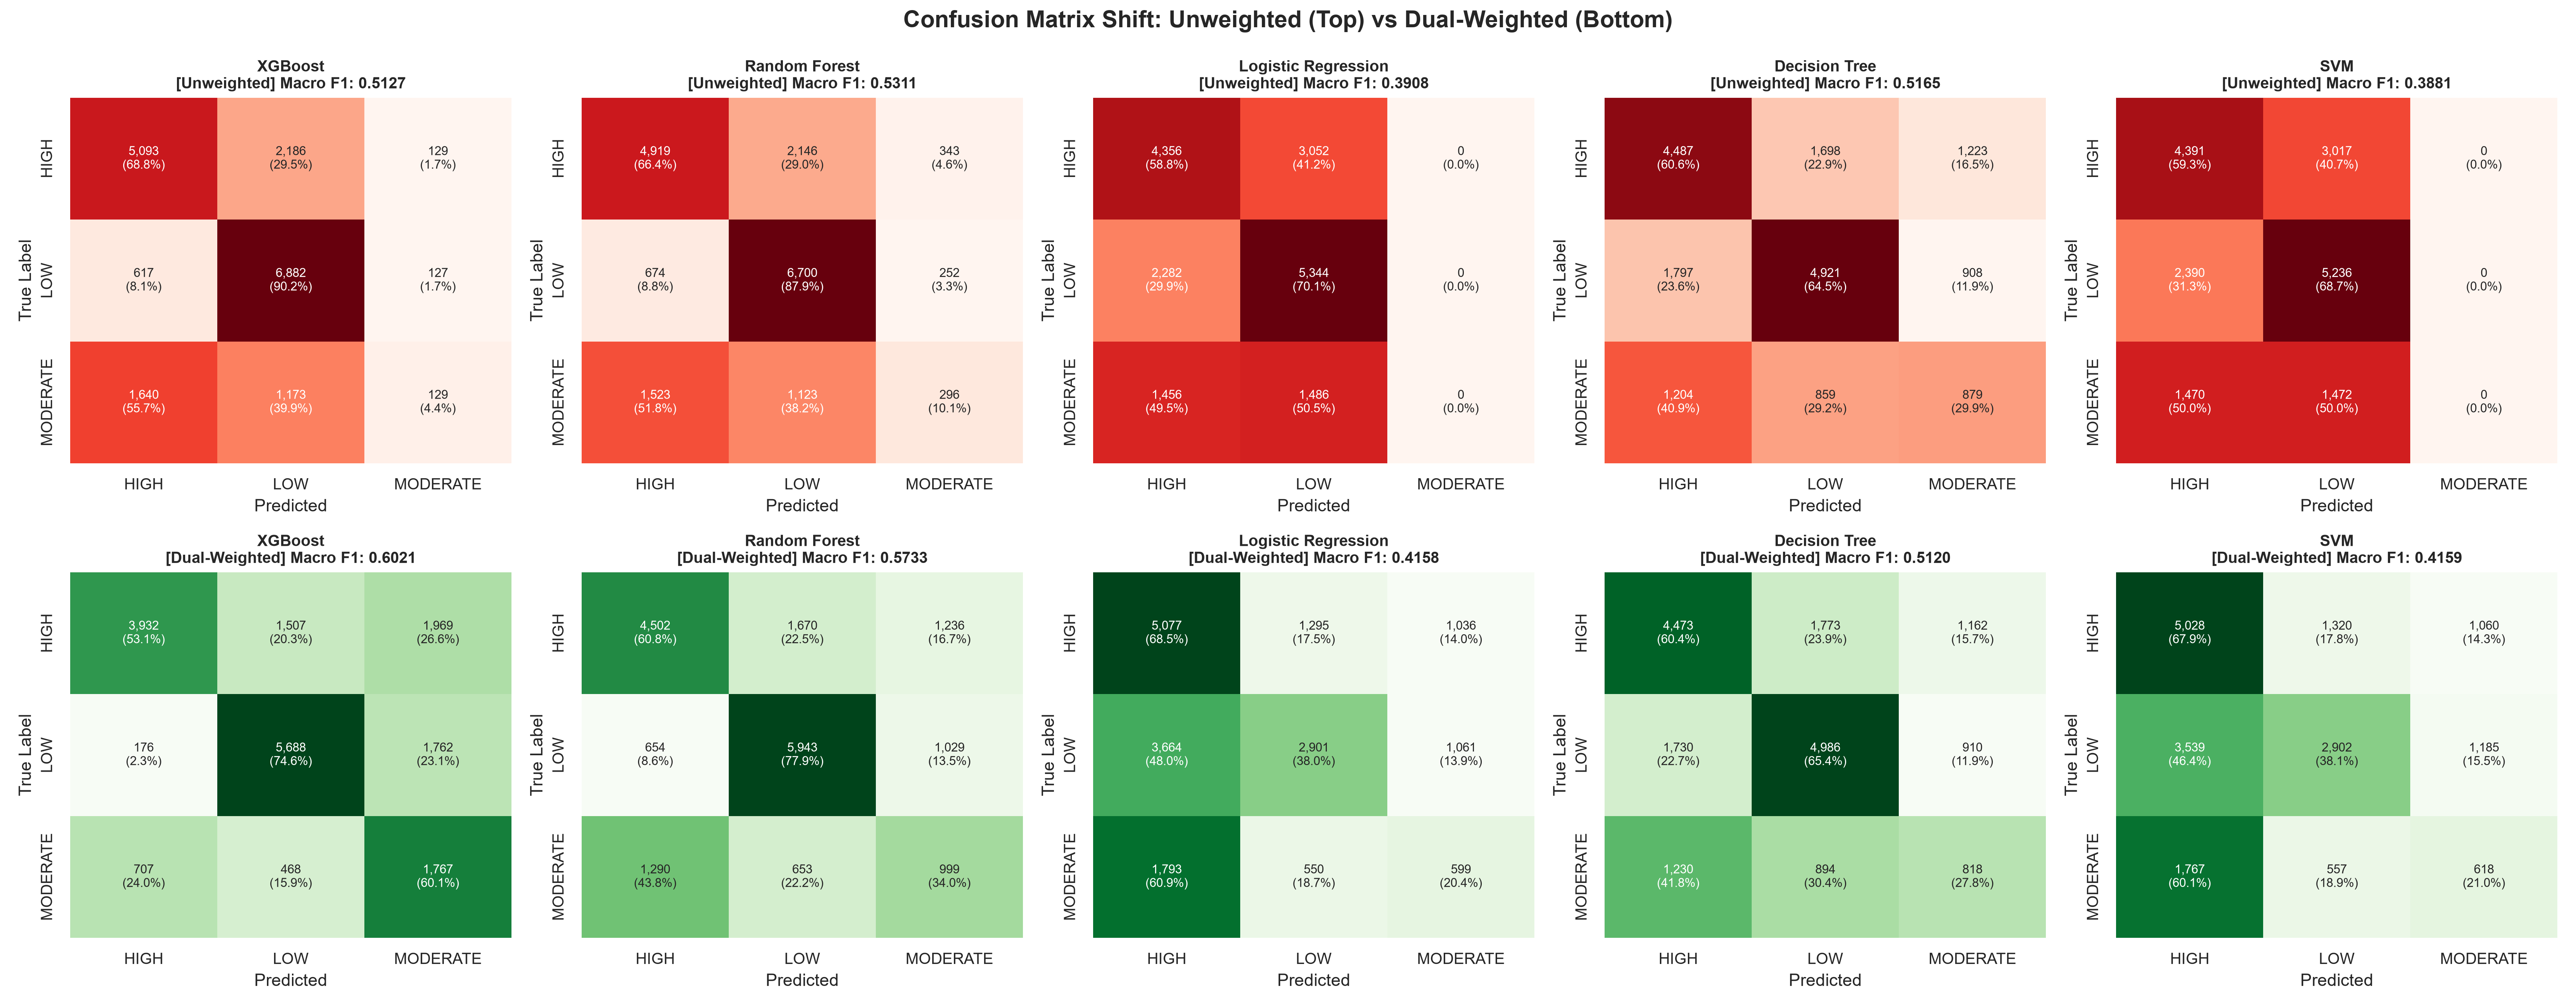
\includegraphics[width=0.98\textwidth]{figures/05_confusion_matrices_unweighted_vs_dual_weighted.png}
    \caption{Correct and incorrect risk predictions for the five models. Extra weighting helps the models identify more MODERATE cases instead of labeling them LOW or HIGH.}
    \label{fig:confusion_matrices_shift}
\end{figure}

The confusion matrices (Figure~\ref{fig:confusion_matrices_shift}) show the trade-off made by dual weighting:
\begin{itemize}[leftmargin=18pt, itemsep=2pt]
    \item \textbf{Operational Trade-off:} HIGH recall shifts from 68.75\% (5,093 caught of 7,408) to 53.08\% (3,932 caught), while HIGH precision rises from 69.29\% to 81.66\%. Fewer HIGH items are flagged as HIGH, but approximately 82\% of HIGH alerts are correct. Crucially, of the 3,476 actual HIGH items not flagged as HIGH, the majority (1,966 receipts, or 56.6\%) are shifted into MODERATE warnings rather than being misclassified as safe LOW stock; meanwhile, severe false-safe errors (actual HIGH misclassified as LOW) dropped substantially from 2,186 to 1,510 receipts.
\end{itemize}

\subsection{Demand Forecast Results}
We tested the demand models on 22,680 observations for each forecast day, covering 2017-07-17 to 2017-08-15. We compared them with a simple baseline that assumes sales will match the same day of the previous week. The models performed better on this test, as shown in Table~\ref{tab:forecast_headline} and Figure~\ref{fig:forecast_wape}.

\begin{table}[H]
\centering
\caption{Demand forecast errors compared with using sales from the same day of the previous week. Lower WAPE means a closer forecast.}
\label{tab:forecast_headline}
\renewcommand{\arraystretch}{1.15}
\setlength{\tabcolsep}{4.5pt}
{\footnotesize
\begin{tabular}{@{} c r r r r r r r @{}}
\toprule
\rowcolor{NavyPrimary}
\color{white}\textbf{Horizon} & \color{white}\textbf{Val WAPE} & \color{white}\textbf{Test MAE} & \color{white}\textbf{Test RMSE} & \color{white}\textbf{Test WAPE} & \color{white}\textbf{Naive MAE} & \color{white}\textbf{Naive WAPE} & \color{white}\textbf{Skill} \\
\midrule
Day +1 & 11.45\% & \textbf{119.02} & \textbf{290.01} & \textbf{12.48\%} & 152.57 & 16.00\% & \textbf{+21.99\%} \\
\rowcolor{LightBg}
Day +2 & 11.79\% & \textbf{122.41} & \textbf{295.74} & \textbf{12.84\%} & 152.57 & 16.00\% & \textbf{+19.77\%} \\
Day +3 & 12.36\% & \textbf{126.02} & \textbf{305.57} & \textbf{13.22\%} & 152.57 & 16.00\% & \textbf{+17.40\%} \\
\bottomrule
\end{tabular}}
\end{table}

\begin{figure}[H]
    \centering
    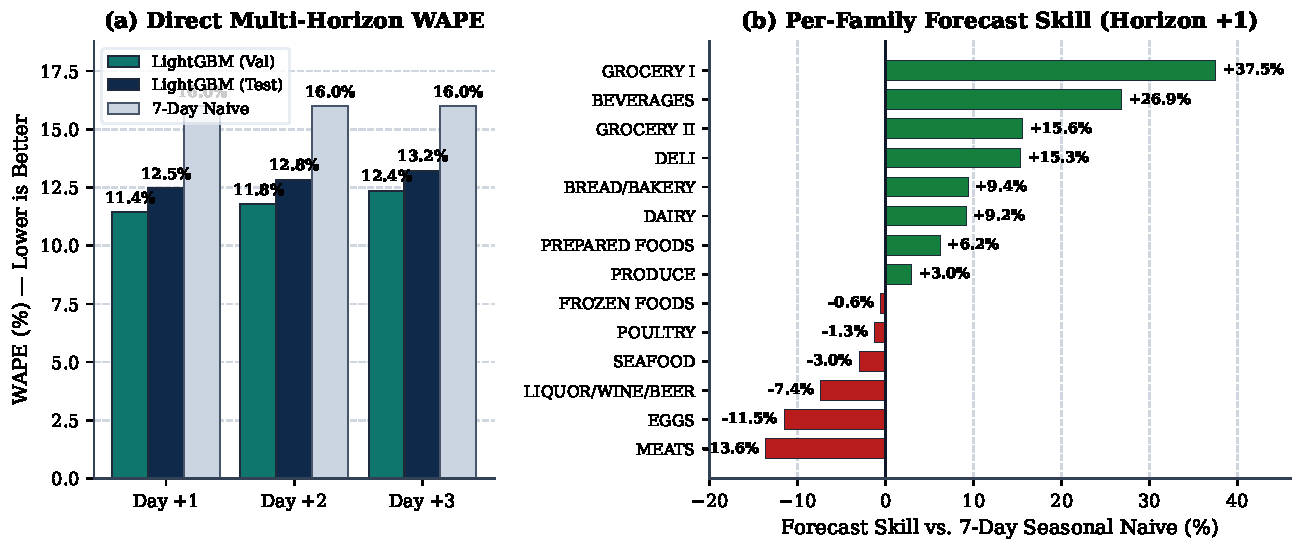
\includegraphics[width=0.98\textwidth]{figures/fig4_forecast_wape_skill.pdf}
    \caption{(a) Forecast error for each day ahead, compared with the validation data and the previous-week baseline. (b) One-day forecast results for each of the 14 food groups.}
    \label{fig:forecast_wape}
\end{figure}

\textbf{Main findings:}
\begin{itemize}[leftmargin=18pt, itemsep=2pt]
    \item \textbf{Forecast error grows slightly with time:} Test error is about one percentage point higher than validation error. WAPE rises from 12.48\% for tomorrow to 13.22\% for three days ahead.
    \item \textbf{Results vary by food group:} The model does best for high-volume groups such as GROCERY I and BEVERAGES. It does less well for some groups with low or irregular sales, such as MEATS, EGGS, and SEAFOOD.
\end{itemize}

\begin{auditnote}[Why the demand forecast is advice only]
The historical demand data is not Malaysian and is divided among products using current stock share, which may overestimate slow-selling items. Forecasts therefore remain unvalidated advice, and automatic purchase orders stay disabled until at least two years of local product-level sales data are collected and checked.
\end{auditnote}

\subsection{Surplus Cargo Regression Model Evaluation}
\label{sec:cargo_regression_results}

When inventory batches are designated for donation or clearance rescue, Module~3 uses a machine-learning regression model to estimate surplus mass (\texttt{Waste\_Quantity} in kilograms), supporting vehicle selection and cold-chain routing.

\subsubsection{Benchmark Setup and Model Hyperparameters}
We benchmarked four regression algorithms on the cleaned food waste repository (8,000 total records), evaluated under an identical 80:20 train/test split (6,400 training samples and 1,600 held-out test samples, random seed 42) with standard feature scaling (\texttt{StandardScaler}) across all 20 engineered features (four numerical and 16 one-hot encoded categories):
\begin{enumerate}[leftmargin=18pt, itemsep=2pt]
    \item \textbf{Linear Regression (Baseline):} Ordinary Least Squares (OLS) regression with intercept fitting.
    \item \textbf{Decision Tree Regressor:} Standard CART regression tree optimized with squared error criterion (\texttt{random\_state=42}).
    \item \textbf{Random Forest Regressor:} Bagging ensemble of 100 regression trees with bootstrap sampling (\texttt{n\_estimators=100}, \texttt{random\_state=42}, parallelized with \texttt{n\_jobs=-1}).
    \item \textbf{XGBoost Regressor (Current Production Model):} Gradient boosted decision trees using the squared error objective, configured with \texttt{n\_estimators=150}, \texttt{learning\_rate=0.08}, \texttt{max\_depth=5}, \texttt{subsample=0.85}, \texttt{colsample\_bytree=0.85}, and \texttt{random\_state=42}.
\end{enumerate}

\subsubsection{Regression Performance Comparison}
Table~\ref{tab:cargo_regression_benchmark} details the comparative evaluation metrics on the 1,600 unseen test records, comprising the coefficient of determination ($R^2$), Mean Absolute Error (MAE), Root Mean Squared Error (RMSE), Mean Squared Error (MSE), and computational training runtime.

\begin{table}[H]
\centering
\caption{Empirical evaluation of surplus cargo regression models on 1,600 held-out test records.}
\label{tab:cargo_regression_benchmark}
\renewcommand{\arraystretch}{1.15}
\setlength{\tabcolsep}{5.5pt}
{\footnotesize
\begin{tabular}{@{} l c c c c c @{}}
\toprule
\rowcolor{NavyPrimary}
\color{white}\textbf{Model Architecture} & \color{white}\textbf{$R^2$ Score} & \color{white}\textbf{MAE (kg)} & \color{white}\textbf{RMSE (kg)} & \color{white}\textbf{MSE} & \color{white}\textbf{Train Time (s)} \\
\midrule
Linear Regression (Baseline) & 0.8005 & 4.238 & 7.807 & 60.952 & \textbf{0.0112} \\
\rowcolor{LightBg}
Decision Tree Regressor & 0.9014 & 1.761 & 5.490 & 30.145 & 0.0363 \\
Random Forest Regressor & 0.9269 & \textbf{1.326} & 4.726 & 22.335 & 0.3011 \\
\rowcolor{LightBg}
\textbf{XGBoost Regressor (Production)} & \textbf{0.9545} & 1.371 & \textbf{3.729} & \textbf{13.903} & 0.3728 \\
\bottomrule
\end{tabular}}
\end{table}

\textbf{Key Insights and Analysis:}
\begin{itemize}[leftmargin=18pt, itemsep=2pt]
    \item \textbf{Cargo Mass Variance Explained ($R^2 = 95.45\%$):} The tuned XGBoost model captures 95.45\% of the variance in surplus cargo weight, significantly outperforming the linear baseline ($R^2 = 80.05\%$) and single decision tree ($R^2 = 90.14\%$).
    \item \textbf{Robustness Against Large-Volume Tail Outliers:} While Random Forest records a marginal advantage in mean absolute deviation (MAE of 1.326~kg vs. 1.371~kg), XGBoost delivers a substantially lower RMSE (3.729~kg vs. 4.726~kg) and reduces MSE by 37.8\% (13.903 vs. 22.335). In logistical operations, large prediction errors carry severe penalties (e.g., dispatching an undersized vehicle that cannot accommodate an evacuation batch). XGBoost's gradient boosting specifically penalizes large residuals, reducing the risk of large errors that could cause an undersized vehicle assignment for bulk donations.
\end{itemize}

% ============================================================================
% SECTION 6: LIMITATIONS & FUTURE WORK
% ============================================================================
\section{What the System Cannot Do Yet}

The system works as a proof of concept, but there are some important limitations. Table~\ref{tab:limitations} explains what they are and what could be improved next.

\begin{table}[H]
\centering
\caption{Current limits of the system and possible improvements.}
\label{tab:limitations}
\renewcommand{\arraystretch}{1.15}
{\scriptsize
\begin{tabularx}{\textwidth}{@{} >{\bfseries}l >{\raggedright\arraybackslash}X >{\raggedright\arraybackslash}X @{}}
\toprule
\rowcolor{NavyPrimary}
\color{white}\textbf{Part of system} & \color{white}\textbf{Current limit} & \color{white}\textbf{Possible next step} \\
\midrule
Demand forecast & The training data is from 2017 and comes from non-Malaysian stores. Splitting group-level forecasts by stock share may overestimate demand for slow-moving products. Some negative predictions are automatically set to zero. & Collect at least two years of Malaysian product-level sales data, then retrain and validate the model before enabling automatic purchase orders. \\
\rowcolor{LightBg}
Malaysian public holidays & Malaysian public holidays are not modelled; demand forecasts do not account for Malaysian holiday effects or festive shopping spikes (e.g., Hari Raya, Chinese New Year, Deepavali). & Ingest historical multi-year Malaysian retail sales data matched with national and state holiday calendars to train localized festive calendar feature embeddings. \\
Spoilage model & The model was trained on historical food records from non-Malaysian stores. While cold-chain deviation and handling quality strongly correlate with spoilage in raw data, they are unrecorded at store receiving docks; the model relies on 19 observable intake features (stock pressure, shelf life, demand, calendar, category). & Equip receiving docks with rapid transit temperature loggers and retrain with Malaysian retail receiving records. \\
\rowcolor{LightBg}
Intake DTE calibration & The 990 demonstration inventory lots were assigned synthetic remaining shelf-lives of 1--12 days relative to the anchor date (\texttt{2026-10-30}) to simulate active retail stock. In production, risk scores depend directly on actual physical expiry dates stamped at receiving docks. & Connect receiving dock barcode/RFID scanners directly to automate physical expiry date entry upon delivery. \\
Store rules & Discount tiers (15\%, 25\%, 50\% fallback) are fixed percentages. Malaysian commodity prices from PriceCatcher are not yet used to dynamically adjust markdown depth based on competitor pricing. & Connect live PriceCatcher price data to dynamically adjust markdown depths, and expand surplus pathways to include animal feed and composting in alignment with ReFED destination frameworks~\cite{refed2026}. \\
\rowcolor{LightBg}
End-to-end baseline comparison & The system lacks empirical comparative trials against an existing FIFO baseline in live operating retail stores; operational benefits are demonstrated through modular algorithmic benchmarks rather than live store-wide A/B testing. & Conduct field pilot studies across partner stores comparing FreshGuard's FEFO-dynamic pricing workflow directly against standard FIFO operations. \\
Dashboard and sales log & Some totals in the dashboard are estimates, and the server and web app calculate them separately. Full-price and discounted sales are grouped under the same event label. & Calculate all totals in one place using recorded events, and tag each sale type separately. \\
\rowcolor{LightBg}
Delivery planning & Each delivery is routed as a single trip from store to food bank. Multi-store pick-ups in the same area are not yet combined. & Add multi-stop routing (Vehicle Routing Problem) to combine pick-ups from several stores in the same area into one trip. \\
\bottomrule
\end{tabularx}}
\end{table}

% ============================================================================
% SECTION 7: CONCLUSION
% ============================================================================
\section{Conclusion}

FreshGuard is a complete working system that connects cleaned inventory data, machine-learning models, food safety rules, delivery routing, and a web dashboard. The dual-weighted XGBoost spoilage model catches more of the hard-to-detect MODERATE-risk cases. The LightGBM demand forecasters consistently outperform a simple previous-week baseline. The cargo regression model estimates donation shipment weight ($R^2 = 95.45\%$), assisting fleet tier allocation.

Food safety is enforced at every step: expired stock is blocked from sale and donation and routed to bio-waste composting. Food that expires today or tomorrow is prioritized for food bank delivery, subject to a 30\% donation cap that prevents stores from over-relying on charity. The web app's adaptive action panel structures clearance workflows by clearly highlighting urgent actions at the top of the decision modal.

FreshGuard demonstrates a practical, end-to-end framework for surplus food management in urban retail environments, although demand forecasts remain advisory until retrained on local Malaysian retail sales data.

% ============================================================================
% REFERENCES
% ============================================================================
\begin{thebibliography}{9}

\bibitem{unep2024}
United Nations Environment Programme (UNEP), \emph{Food Waste Index Report 2024: Think Eat Save --- Tracking Global Food Waste to Halve It by 2030}, Nairobi, Kenya, 2024. Available: \url{https://www.unep.org/resources/publication/food-waste-index-report-2024}

\bibitem{refed2026}
ReFED, \emph{ReFED Food Waste Measurement Framework and Surplus Destination Taxonomy}, Technical Report, 2026. Available: \url{https://refed.org/downloads/2026-refed-measurement-report.pdf}

\bibitem{chen2016xgboost}
T.~Chen and C.~Guestrin, ``XGBoost: A Scalable Tree Boosting System,'' in \emph{Proceedings of the 22nd ACM SIGKDD International Conference on Knowledge Discovery and Data Mining (KDD '16)}, San Francisco, CA, USA, pp.~785--794, 2016.

\bibitem{ke2017lightgbm}
G.~Ke, Q.~Meng, T.~Finley, T.~Wang, W.~Chen, W.~Ma, Q.~Ye, and T.-Y.~Liu, ``LightGBM: A Highly Efficient Gradient Boosting Decision Tree,'' in \emph{Advances in Neural Information Processing Systems (NeurIPS)}, vol.~30, pp.~3146--3154, 2017.

\bibitem{dosm2026}
Department of Statistics Malaysia (OpenDOSM), \emph{PriceCatcher Daily Retail Commodity Price Dataset}, Open Government Data Portal, CC BY 4.0. Available: \url{https://open.dosm.gov.my/data-catalogue/pricecatcher}

\bibitem{osrm}
Project OSRM, \emph{Open Source Routing Machine --- High-Performance Routing Engine for Shortest Paths in Road Networks}. Available: \url{https://github.com/Project-OSRM}

\end{thebibliography}

\end{document}
